\documentclass[12pt]{article}
\usepackage[margin=1.0in]{geometry}
\usepackage{graphicx}
\bibliographystyle{plain}
\usepackage{mathtools}
\usepackage{subfigure}

\begin{document}

\section{Specific Aim 2.1}

SET domain protein models of SETD2 and NSD2 were built using Modeller with PDBs 4FMU and 3OOI as inputs, respectively.  Proteins were placed in TIP3P water boxes of approximately 7 nm, with NaCl ions added to achieve neutrality.  The ff99sb-ildn force field \cite{} was used.  Systems were held at constant temperature (300K) and pressure (1 atmosphere) using a Langevin integrator and Monte Carlo barostat, as implemented in OpenMM 6.0.1 \cite{}.  For each system, a total of 50-100 $\mu s$ of simulations was analyzed using MDTraj \cite{}, MSMBuilder \cite{}, and Mixtape \cite{}.  Slow coordinates were selected using temporal independent component analysis (tICA) \cite{} with randomly selected geometric features as inputs.  Seven-state Markov state models were constructed by Gaussian Mixture Model clustering of the two slowest linear combinations of features.

\begin{figure}
\subfigure[]{
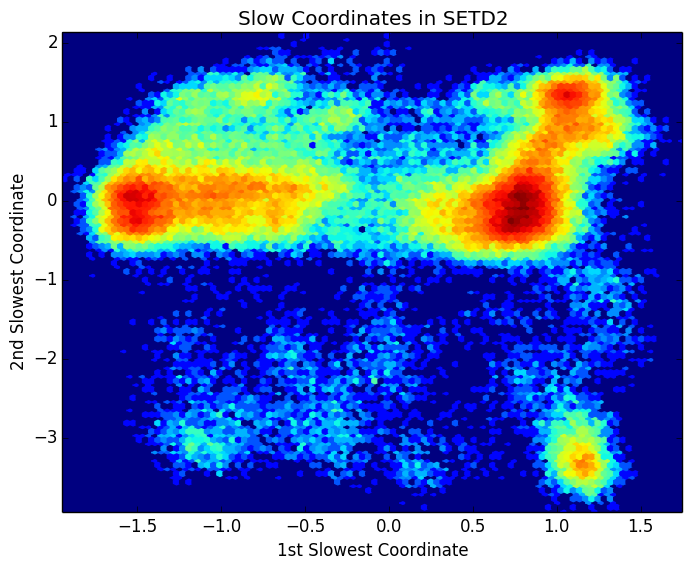
\includegraphics[width=5.0cm]{figures/SETD2_tics.png}
}
\subfigure[]{
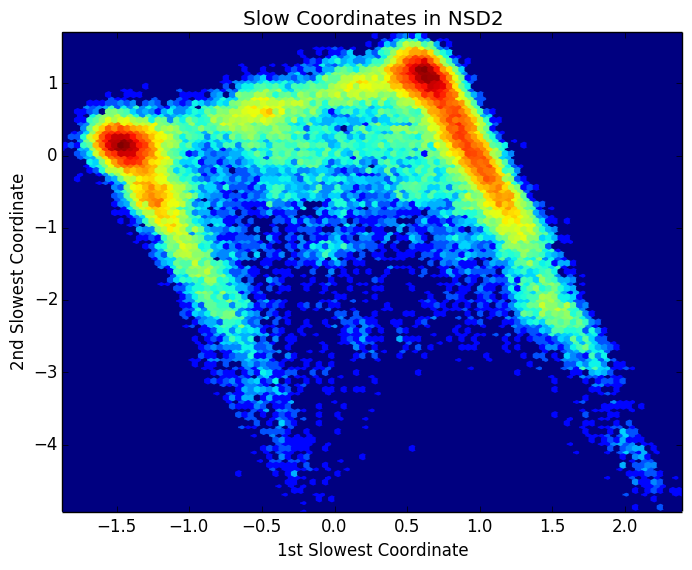
\includegraphics[width=5.0cm]{figures/NSD2_tics.png}
}


\subfigure[]{
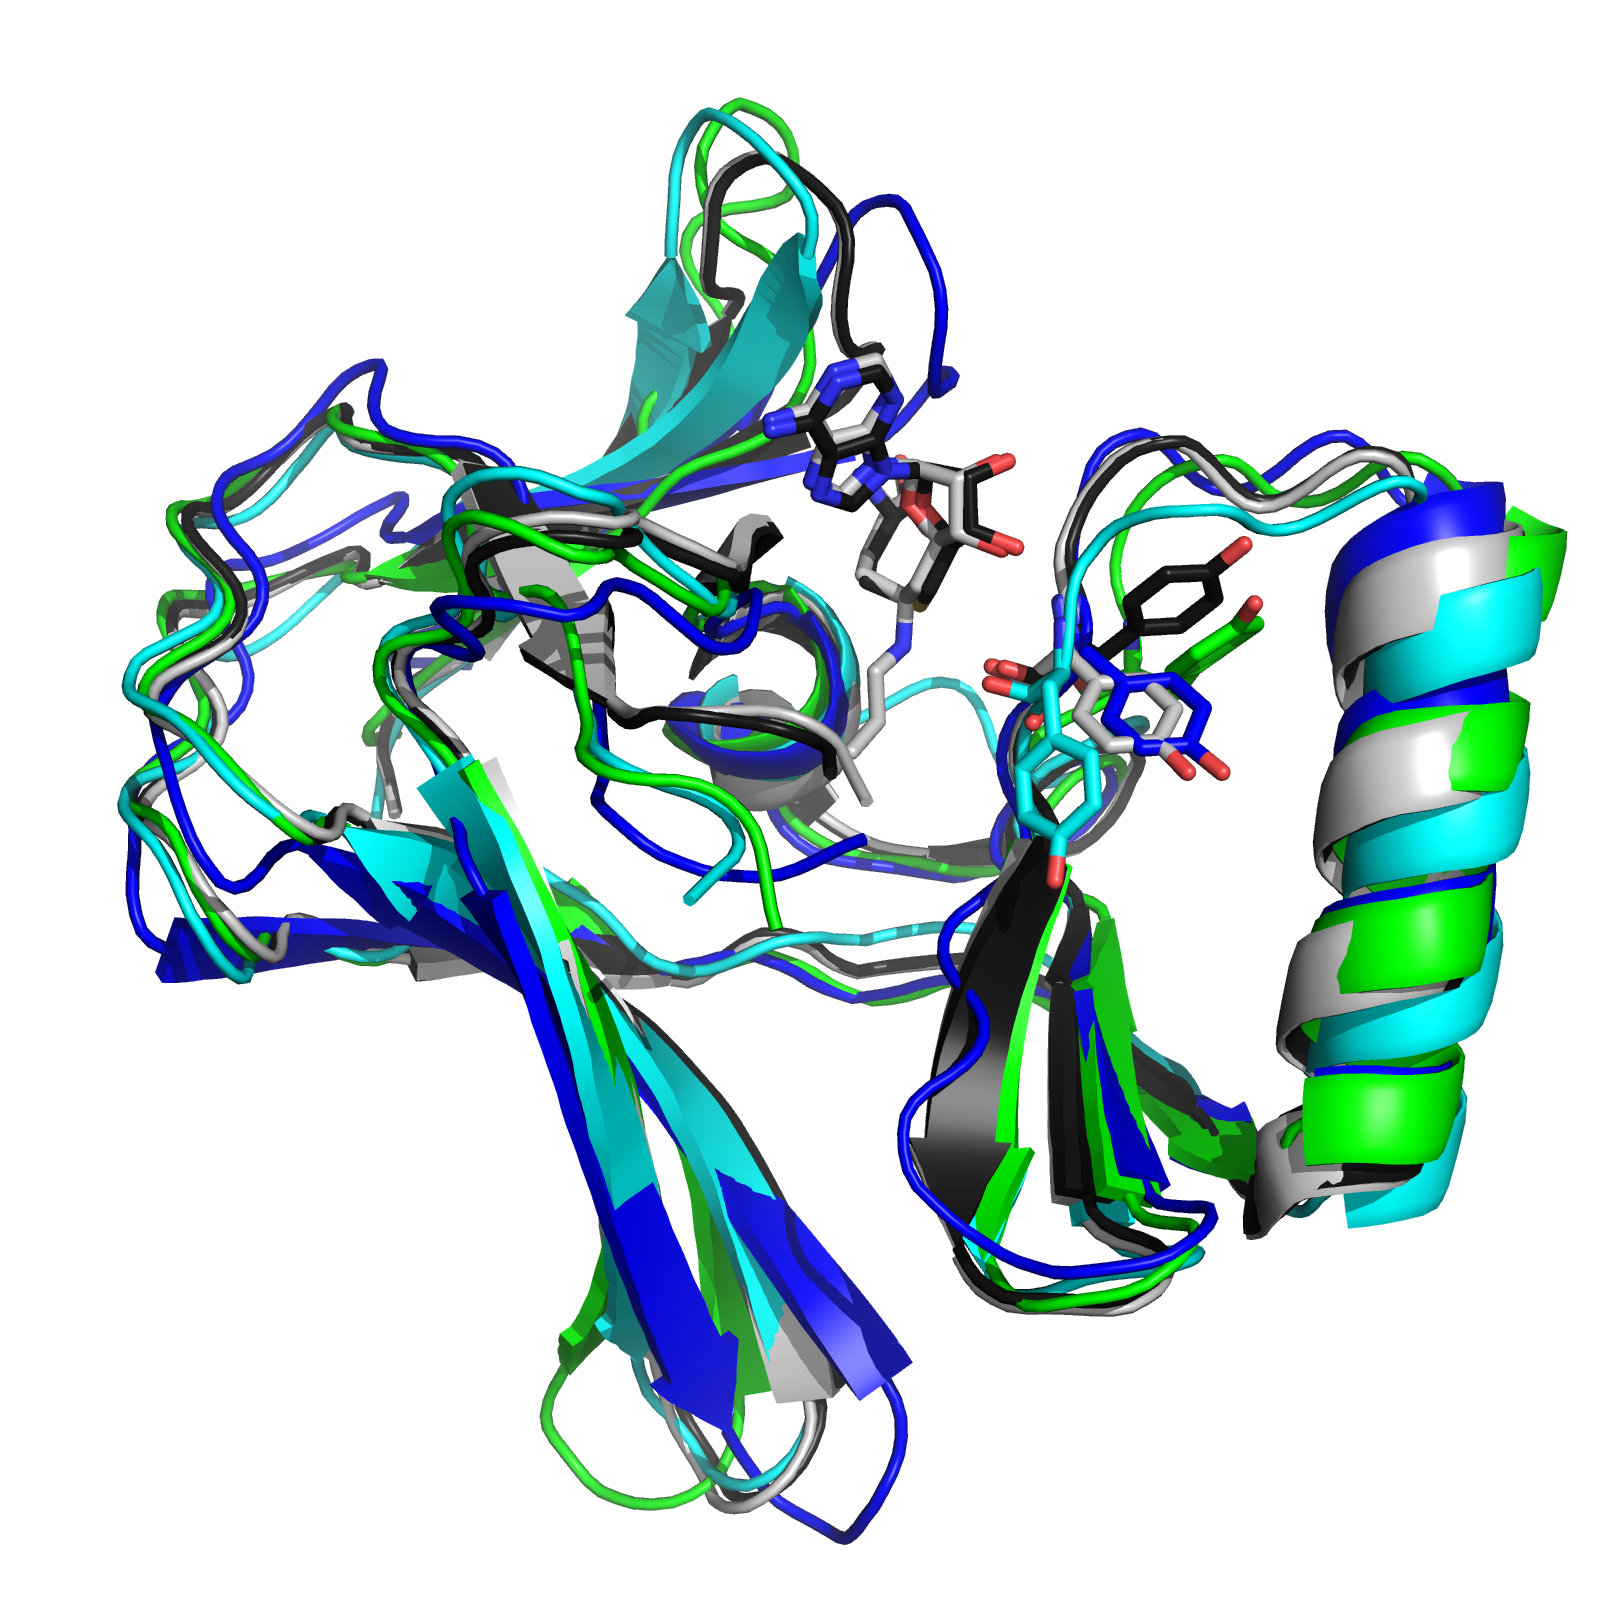
\includegraphics[width=5.0cm]{figures/SETD2_pdb.png}
}
\subfigure[]{
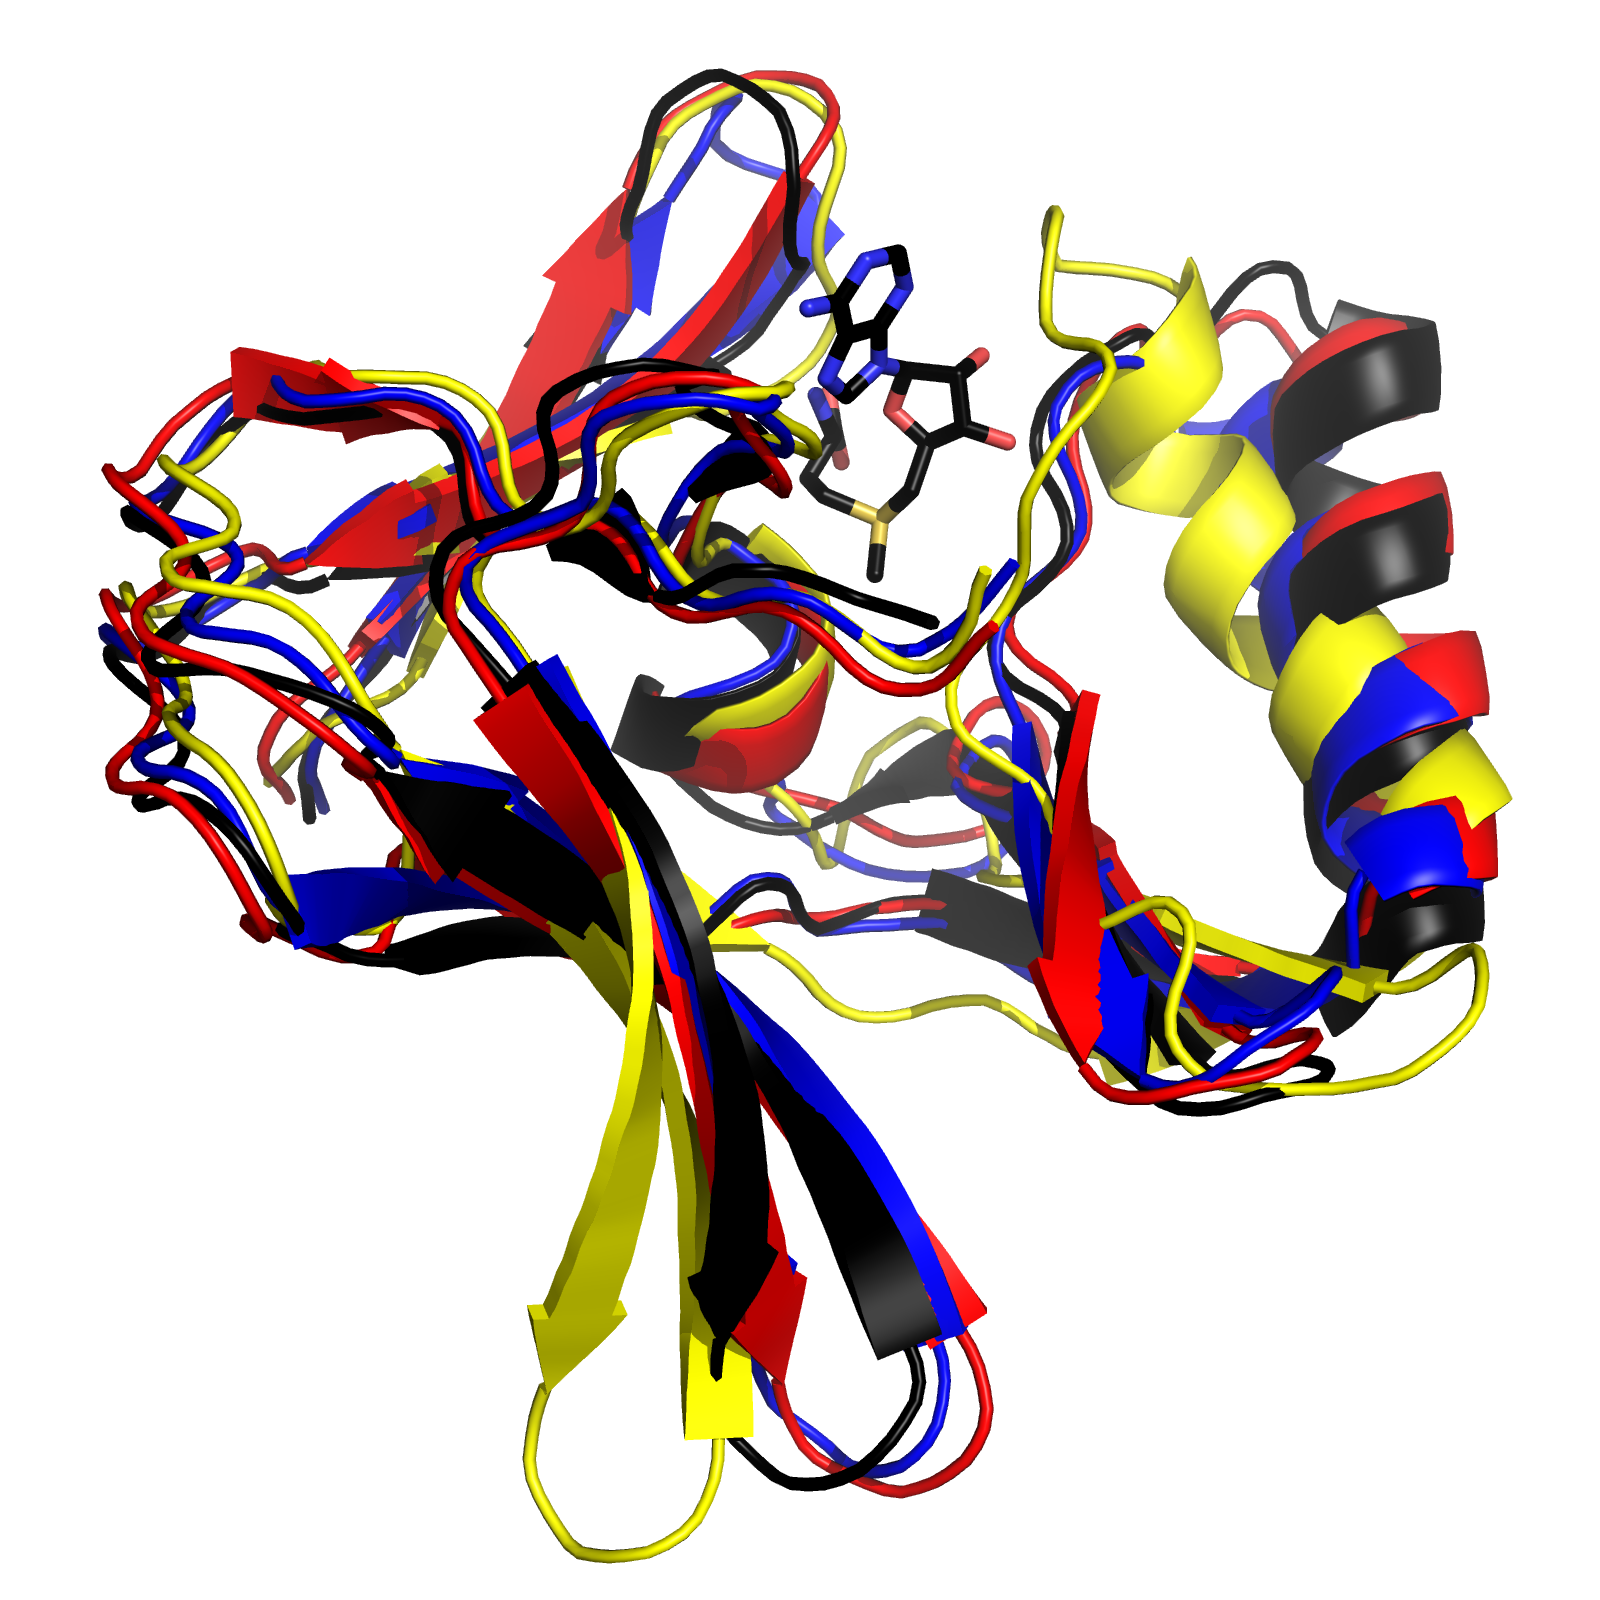
\includegraphics[width=5.0cm]{figures/NSD2_pdb.png}
}

\caption{
(a, b).  Conformational landscapes---projections onto the two slowest coordinates---show multiple heterogeneous conformational states observed in simulations at the ~$50 \mu s$ timescale.  (c, d). Structural comparisons indicate conformational heterogeneity near the known SAM / sinefungin binding site.  Ligand-bound crystal structures (pink, cyan) show similar conformational states.  Panels a and c correspond to SETD2, while panels b and d correspond to NSD2.  SETD2 bound to SAH (d: cyan) adopts a TYR-up orientation (PDB:4H12), while SETD2 bound to sinefungin (d: pink) adopts a TYR-down orientation (PDB:4HMU).  NSD1 bound to SAM (e: pink) adopts a PHE-up conformation (PDB: 3OOI).  In all three systems, simulations suggest the presence of both conformations in solution, suggesting that predictive models of binding affinity and selectivity will require careful accounting for the conformational preferences of the unbound protein.  In particular, our models predict similar conformational states in NSD2, for which there is currently no crystal structure.
}
\label{figure:MSM}
\end{figure}


\end{document}
